\documentclass[11pt,a4paper]{article}
\usepackage[T1]{fontenc}
\usepackage[utf8]{inputenc}
\usepackage{lmodern}
\usepackage{microtype}
\usepackage[margin=27mm]{geometry}
\usepackage{amsmath,amssymb,amsfonts,amsthm,mathtools}
\usepackage{booktabs,graphicx,enumitem,array}
\usepackage[colorlinks=true,linkcolor=black,citecolor=black,urlcolor=blue]{hyperref}
\usepackage{cleveref}
\allowdisplaybreaks[2]
\hypersetup{pdftitle={Exact Triaxial Spin-4 Stability Thresholds for an Anisotropic SU(2) Quadratic Operator},pdfauthor={Africa Compute Fund Research Programme},pdfsubject={Technical preprint on exact SU(2) finite-spin spectral thresholds},pdfkeywords={SU(2), spin-4, triaxial, stability thresholds, symbolic verification}}
\setlength{\parskip}{0.35em}
\setlength{\parindent}{0pt}
\newtheorem{theorem}{Theorem}[section]
\newtheorem{proposition}[theorem]{Proposition}
\newtheorem{lemma}[theorem]{Lemma}
\newtheorem{corollary}[theorem]{Corollary}
\newtheorem{remark}[theorem]{Remark}
\newcommand{\qs}{Q_s(c)}
\newcommand{\J}{J}
\title{\bfseries Exact Triaxial Spin-4 Stability Thresholds\\[3pt]
for an Anisotropic $\mathrm{SU}(2)$ Quadratic Operator}
\author{Africa Compute Fund\\\small Research Programme}
\date{Technical preprint \quad\textbullet\quad 3 November 2026}
\begin{document}
\maketitle
\begin{abstract}
\emergencystretch=2em
For the integer-spin irreducible representations of $\mathfrak{su}(2)$, we study the
positive-definiteness threshold of the Hermitian quadratic operator
$Q_s(c)=aJ_1^2+bJ_2^2-cJ_3^2$, with $a\geq b>0$ and $c\geq0$.
We factor the spin-four determinant exactly, identify its first positive zero
uniformly over the full anisotropy domain, and obtain a closed radical formula
for the threshold $c_4$. An independent factor analysis also yields a closed
spin-three threshold $c_3$. Exact resultant and sign arguments establish
$c_4<c_3<c_2<c_1$ for every $a\geq b>0$, including the isotropic boundary.
For arbitrary integer spin $s\geq1$, a separate variational estimate gives
$b/s\leq c_s\leq(a+b)/(2s)$, proving that fixed $c>0$ cannot preserve
positive definiteness throughout an unbounded tower of these pure quadratic
blocks. All finite-spin determinant identities and comparison certificates
are accompanied by an executable, independently reconstructed symbolic and
numerical reproducer. The statements concern this specified matrix family;
they do not establish a physical fluctuation spectrum or the viability of a
particular matrix-model background.
\end{abstract}

\textbf{Keywords:} angular momentum; anisotropic quadratic operators;
finite-dimensional spectral theory; exact algebraic thresholds; symbolic
verification; matrix models.

\section{Introduction}
Anisotropic quadratic forms in angular-momentum generators appear in the
spectral theory of quantum asymmetric tops, collective-spin systems and
related matrix models. Their algebraic structure is well established; see,
for example, the asymmetric-top treatment of Breev and Gitman
\cite{breev2023}, the collective-spin perspective of Opatrn\'{y}
\emph{et al.}\ \cite{opatrny2018}, and the exact-spectrum analysis of
Ribeiro, Vidal and Mosseri \cite{ribeiro2008}. A negative coefficient
in such a quadratic form changes a precise mathematical question: when
does its spectrum first reach zero?

We address that question for a fixed family of finite-dimensional
Hermitian matrices and a specified coefficient domain. The primary
object is the first loss of \emph{strict positive definiteness}, not a
dynamical growth exponent or an experimentally demonstrated
instability. The distinction is essential: a physical system can have
additional Hessian terms, constraints, gauge or ghost sectors, and
spin-dependent coefficients absent from the operator studied here.

The concrete results are: (i) an explicit spin-four determinant and its
globally minimal factor root; (ii) a closed spin-three formula and a
strict ordering of all four integer-spin thresholds; and (iii) an
all-spin variational envelope. Proofs use exact polynomial identities,
nonvanishing resultants, rational root isolation and the
Rayleigh--Ritz principle. We make no claim of priority for the general operator class,
the standard variational technique, or an exhaustively established
novelty assessment.

\section{Operator, notation and meaning of the threshold}\label{sec:setup}
For integer $s\geq1$, let $J_1,J_2,J_3$ be the Hermitian generators
of the spin-$s$ irreducible representation, acting on
$\mathcal H_s\cong\mathbb C^{2s+1}$. Our conventions are
\begin{equation}\label{eq:su2}
[J_i,J_j]=i\varepsilon_{ijk}J_k,\qquad
J_1^2+J_2^2+J_3^2=s(s+1)I.
\end{equation}
In the $J_3$ eigenbasis, $m=-s,-s+1,\ldots,s$,
\begin{align}
J_3|s,m\rangle&=m|s,m\rangle,\label{eq:z}\\
J_\pm|s,m\rangle&=\sqrt{(s\mp m)(s\pm m+1)}
\,|s,m\pm1\rangle,\label{eq:ladder}
\end{align}
where $J_\pm=J_1\pm iJ_2$.

Throughout the paper,
\begin{equation}\label{eq:Q}
Q_s(c):=aJ_1^2+bJ_2^2-cJ_3^2,
\qquad a\geq b>0,\quad c\geq0.
\end{equation}
We write $A\succ0$ for strict positive definiteness and use the
following unambiguous definition:
\begin{equation}\label{eq:thresholddef}
c_s(a,b):=\inf\{c\geq0:Q_s(c)\not\succ0\}.
\end{equation}
The spin-zero block is excluded because $Q_0(c)=0$ identically.
By homogeneity, $c_s(a,b)=b\,x_s(r)$ for
\begin{equation}\label{eq:scaling}
r:=a/b\geq1,\qquad x:=c/b.
\end{equation}
A zero of $\det Q_s(c)$ is a threshold candidate; identifying the
\emph{first} zero and proving positivity on its left are separate steps.

\begin{lemma}[Initial positivity and monotonicity]\label{lem:monotone}
For every integer $s\geq1$, $Q_s(0)\succ0$ and
$\lambda_{\min}(Q_s(c))$ is nonincreasing in $c$. Consequently,
$c_s$ is the smallest nonnegative determinant zero and
$Q_s(c)\succ0$ exactly when $0\leq c<c_s$.
\end{lemma}
\begin{proof}
For any $v$,
$\langle v,Q_s(0)v\rangle\geq
b(\|J_1v\|^2+\|J_2v\|^2)$.
If this vanishes, then $J_1v=J_2v=0$ and hence
$J_3v=(1/i)[J_1,J_2]v=0$. The Casimir identity
\eqref{eq:su2} then forces $s(s+1)v=0$, so $v=0$.
For $c'\geq c$, $Q_s(c')-Q_s(c)=-(c'-c)J_3^2\preceq0$.
The Rayleigh--Ritz characterization of the least eigenvalue
proves monotonicity. Since the highest-weight expectation tends
to $-\infty$ as $c\to\infty$, a threshold exists and is
positive; continuity and monotonicity complete the argument.
\end{proof}

Expanding \eqref{eq:Q} in ladder operators gives a useful sparse
form valid for every integer $s$:
\begin{align}
\langle s,m|Q_s(c)|s,m\rangle
 &=\frac{a+b}{2}\,[s(s+1)-m^2]-cm^2,\label{eq:diag}\\
\langle s,m+2|Q_s(c)|s,m\rangle
 &=\frac{a-b}{4}
\sqrt{(s-m)(s+m+1)(s-m-1)(s+m+2)}.\label{eq:offdiag}
\end{align}
All other off-diagonal entries vanish. Thus the even-$m$ and odd-$m$
subspaces are invariant, and the determinants factor into small
polynomial blocks.

\section{Exact spin-four threshold}\label{sec:spin4}
Let $s=4$, so that $\dim\mathcal H_4=9$.
An exact determinant evaluation using \eqref{eq:diag}--\eqref{eq:offdiag}
gives
\begin{equation}\label{eq:det4}
\det Q_4(c)=320F_1F_2F_3F_4,
\end{equation}
where
\begin{align}
F_1&=2(a+b)c^2-(2a^2+13ab+2b^2)c+2ab(a+b),\label{eq:F1}\\
F_2&=64c^2-136(a+b)c+9a^2+46ab+9b^2,\label{eq:F2}\\
F_3&=9c^2-(46a+136b)c+9a^2+136ab+64b^2,\label{eq:F3}\\
F_4&=9c^2-(136a+46b)c+64a^2+136ab+9b^2.\label{eq:F4}
\end{align}
These are exact polynomial identities, not numerical interpolations.
The $c$-degree is eight rather than nine because the $m=0$ basis
vector has zero $J_3^2$ expectation.

\begin{theorem}[Global spin-four first crossing]\label{thm:spin4}
For every $a\geq b>0$, the first positive determinant zero of
$Q_4$ is the smaller root of $F_1$. In particular, with
\begin{equation}\label{eq:BD}
B=2a^2+13ab+2b^2,
\qquad \Delta=B^2-16ab(a+b)^2,
\end{equation}
its positive-definiteness threshold is
\begin{equation}\label{eq:c4}
\boxed{
 c_4=\frac{B-\sqrt\Delta}{4(a+b)}
 =\frac{4ab(a+b)}{B+\sqrt\Delta}.}
\end{equation}
For $a>b$ this root is strictly smaller than the positive
roots of $F_2,F_3,F_4$. When $a=b$, the least roots of
$F_1$ and $F_2$ coincide.
\end{theorem}
\begin{proof}
Use \eqref{eq:scaling} and denote by $F_i(r,x)$ the
polynomials \eqref{eq:F1}--\eqref{eq:F4} with $a=r,b=1,c=x$.
Their quadratic discriminants are respectively
\begin{align*}
D_1&=4r^4+36r^3+145r^2+36r+4,\\
D_2&=64(253r^2+394r+253),\\
D_3&=64(28r^2+119r+253),\\
D_4&=64(253r^2+119r+28).
\end{align*}
For $r\geq1$ these are strictly positive; each quadratic has
positive leading and constant terms and a negative linear
coefficient. Both roots of each factor are therefore distinct
and positive, with smaller branches continuous in $r$.

The exact resultants, eliminating $x$, are
\begin{align}
\operatorname{Res}_x(F_1,F_2)&=-2268(r-1)^6,\nonumber\\
\operatorname{Res}_x(F_1,F_3)&=-63(r+4)^4(4r+1)^2,\label{eq:res4}\\
\operatorname{Res}_x(F_1,F_4)&=-63(r+4)^2(4r+1)^4.\nonumber
\end{align}
They never vanish for $r>1$; no root of $F_1$ can meet a root
of another factor there. At the exact rational point $r=2$,
positive-to-negative sign changes below each quadratic vertex
isolate the smaller positive roots in
\begin{equation}\label{eq:intervals4}
\begin{aligned}
x_{1,-}&\in(354/1000,355/1000),&
x_{2,-}&\in(355/1000,356/1000),\\
x_{3,-}&\in(1752/1000,1754/1000),&
x_{4,-}&\in(1777/1000,1779/1000).
\end{aligned}
\end{equation}
The $F_1$ smaller root is strictly left of the others.
Continuity and \eqref{eq:res4} preserve that order for all $r>1$.
At $r=1$, $F_1$ and $F_2$ have roots $\{1/4,4\}$, while
$F_3$ and $F_4$ have roots $\{11/9,19\}$.
The earliest zero is therefore always the smaller $F_1$ root.
Solving \eqref{eq:F1} and rationalizing gives \eqref{eq:c4};
\cref{lem:monotone} identifies it as the threshold.
\end{proof}

The rationalized expression in \eqref{eq:c4} is numerically
preferable when $a/b$ is large because it avoids cancellation
in $B-\sqrt\Delta$.

\section{Exact thresholds at spins one, two and three}\label{sec:lower}
The lower-spin determinants may also be built directly from the
ladder matrices. With $r=a/b$ and $x=c/b$,
\begin{align}
\frac{\det Q_1}{b^3}
 &=(r+1)(r-x)(1-x),\label{eq:det1}\\
\frac{\det Q_2}{b^5}
 &=12(r+1-4x)(r+4-x)(4r+1-x)
       [r-(r+1)x],\label{eq:det2}\\
\frac{\det Q_3}{b^7}
 &=108g_1g_2g_3g_4,\label{eq:det3}
\end{align}
with
\begin{align}
g_1&=r+1-x,\\
g_2&=3r^2+8r-(26r+8)x+3x^2,\\
g_3&=3r^2+26r+3-8(r+1)x,\\
g_4&=8r+3-(8r+26)x+3x^2.
\end{align}
It follows immediately that
\begin{equation}\label{eq:c12}
\boxed{c_1=b,\qquad c_2=\frac{ab}{a+b}.}
\end{equation}
Indeed $r/(r+1)\leq(r+1)/4$ because $(r-1)^2\geq0$,
and the other spin-two roots are larger.

\begin{proposition}[Closed spin-three threshold]\label{prop:spin3}
For every $a\geq b>0$, the first positive spin-three zero is
the smaller root of $g_4$, namely
\begin{equation}\label{eq:c3}
\boxed{c_3=b\,\frac{4r+13-4\sqrt{r^2+5r+10}}{3}
 =b\,\frac{8r+3}{4r+13+4\sqrt{r^2+5r+10}}},
\qquad r=a/b.
\end{equation}
The competing smaller root of $g_2$ is equal to this value
at $a=b$, but strictly larger when $a>b$.
\end{proposition}
\begin{proof}
The two roots of each of $g_2,g_4$ are positive and distinct
for $r\geq1$: their respective discriminants are
$64(10r^2+5r+1)$ and $64(r^2+5r+10)$.
The roots of the two linear factors $g_1,g_3$ are positive.
The exact resultants are
\begin{align}
\operatorname{Res}_x(g_4,g_1)&=-5(r+2)^2,\nonumber\\
\operatorname{Res}_x(g_4,g_2)&=-1215(r-1)^4,\label{eq:res3}\\
\operatorname{Res}_x(g_4,g_3)&=-15(r+3)^3(11r+1).\nonumber
\end{align}
They are nonzero on $r>1$. At $r=2$, exact rational sign
changes below the quadratic vertices isolate the least roots:
\[
x_{g_4,-}\in(468/1000,469/1000),\qquad
x_{g_2,-}\in(478/1000,479/1000).
\]
The linear factors $g_3$ and $g_1$ vanish at $67/24$ and $3$.
Thus $g_4$ has the earliest zero. As none of these roots can
cross those of $g_4$ for $r>1$,
its smaller root is globally first. At $r=1$, the least roots
of $g_2$ and $g_4$ coincide at $1/3$; the other factors first
vanish at $2$. The quadratic formula, with its rationalized
variant, gives \eqref{eq:c3}.
\end{proof}

\section{Global threshold ordering for the finite tower}\label{sec:order}
\begin{theorem}[Strict order through spin four]\label{thm:order}
For every $a\geq b>0$, the positive-definiteness thresholds
of the four integer-spin blocks satisfy
\begin{equation}\label{eq:chain}
\boxed{0<c_4<c_3<c_2<c_1.}
\end{equation}
Consequently, the direct sum $\bigoplus_{s=1}^4Q_s(c)$ is
strictly positive definite if and only if $0\leq c<c_4$.
\end{theorem}
\begin{proof}
By \cref{thm:spin4,prop:spin3}, the relevant first roots are the
smaller roots of $F_1$ and $g_4$. The exact resultant
\begin{equation}\label{eq:res43}
\operatorname{Res}_x(F_1,g_4)
=-(320r^4+928r^3+1703r^2+120r+240)
\end{equation}
is strictly negative for every $r\geq1$. Both smaller roots
are continuous in $r$, and at $r=1$ they are $1/4$ and
$1/3$, respectively. They cannot cross, so $c_4<c_3$
for the entire domain.

Next, with $x_2=r/(r+1)$,
\begin{equation}\label{eq:signg4}
g_4(0)=8r+3>0,
\qquad
g_4(x_2)=-\frac{3(4r^2+4r-1)}{(r+1)^2}<0.
\end{equation}
By continuity, the first $g_4$ zero precedes $x_2$,
so $c_3<c_2$. Finally $r/(r+1)<1$, giving $c_2<c_1$.
Initial positivity and \cref{lem:monotone} establish the direct-sum
criterion.
\end{proof}

\begin{figure}[t]
  \centering
  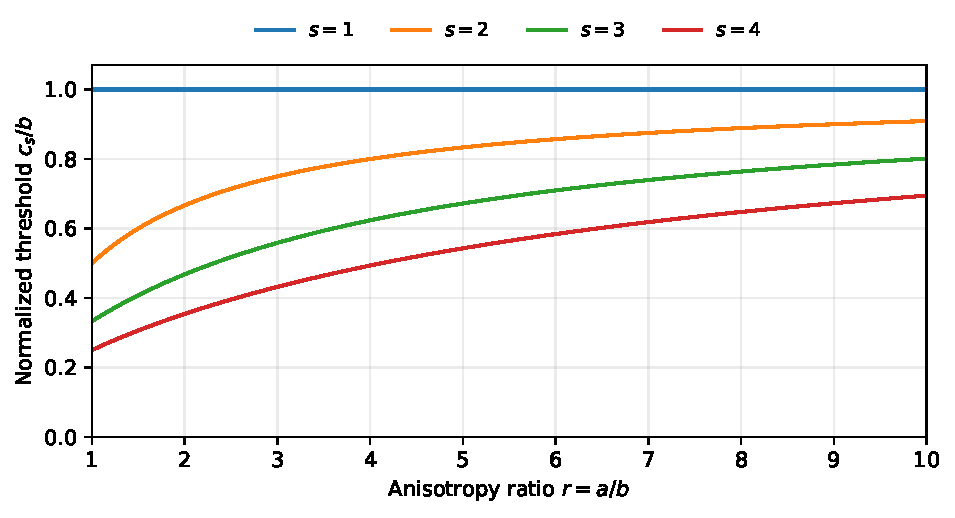
\includegraphics[width=.94\linewidth]{thresholds.pdf}
  \caption{Dimensionless thresholds $x_s=c_s/b$ versus $r=a/b$
  for the exact integer-spin sectors $s=1,2,3,4$.
  The plotted curves are evaluations of the analytical formulas,
  not evidence for a theorem beyond these four sectors.}
  \label{fig:thresholds}
\end{figure}

\begin{table}[t]
\centering
\caption{Representative thresholds from the closed formulas.
Rows test the isotropic boundary and several anisotropic points.}
\label{tab:examples}
\begin{tabular}{@{}ccrrrr@{}}
\toprule
$a$ & $b$ & $c_1$ & $c_2$ & $c_3$ & $c_4$\\
\midrule
1 & 1 & 1.000000 & 0.500000 & 0.333333 & 0.250000\\
2 & 1 & 1.000000 & 0.666667 & 0.468027 & 0.354249\\
3 & 2 & 2.000000 & 1.200000 & 0.815741 & 0.613062\\
5 & 1 & 1.000000 & 0.833333 & 0.672044 & 0.543069\\
10 & 9 & 9.000000 & 4.736842 & 3.162430 & 2.371925\\
\bottomrule
\end{tabular}
\end{table}

\section{An all-spin variational envelope}\label{sec:allspin}
The proof of \cref{thm:order} stops at spin four. A different,
elementary argument yields nontrivial information for every
integer spin without assuming that adjacent-spin thresholds
remain ordered.

\begin{theorem}[All-spin threshold bounds]\label{thm:bounds}
For any integer $s\geq1$ and fixed $a\geq b>0$,
\begin{equation}\label{eq:envelope}
\boxed{\frac b s\leq c_s(a,b)\leq\frac{a+b}{2s}.}
\end{equation}
The bounds coincide at $a=b$, where $c_s=b/s$.
In particular, $c_s(a,b)\to0$ as $s\to\infty$.
For any fixed $c>0$, the collection of all integer-spin
pure quadratic blocks $\{Q_s(c):s\geq1\}$ cannot remain
positive definite.
\end{theorem}
\begin{proof}
Since $a\geq b$, the Casimir identity yields
\begin{align*}
Q_s(c)&\succeq b(J_1^2+J_2^2)-cJ_3^2\\
&=bs(s+1)I-(b+c)J_3^2\\
&\succeq [bs(s+1)-(b+c)s^2]I,
\end{align*}
using $J_3^2\preceq s^2I$. The last scalar is strictly
positive when $c<b/s$, proving the lower bound.
On the normalized highest-weight vector $|s,s\rangle$,
$\langle J_1^2\rangle=\langle J_2^2\rangle=s/2$ and
$\langle J_3^2\rangle=s^2$. Hence
\[
\langle s,s|Q_s(c)|s,s\rangle
=\frac{s(a+b)}2-cs^2.
\]
This expectation is negative for $c>(a+b)/(2s)$; the
Rayleigh--Ritz principle gives the upper bound. At $a=b$,
$Q_s(c)=bs(s+1)I-(b+c)J_3^2$ is diagonal and its
first zero occurs at $|m|=s$ and $c=b/s$.
The limit and nonuniform-positivity conclusion follow from
\eqref{eq:envelope}.
\end{proof}

\begin{remark}
\Cref{thm:bounds} does \emph{not} establish
$c_{s+1}<c_s$ for all $s$ and says nothing about a physical
unbounded tower with extra operators, gauge constraints,
finite cutoffs, or spin-dependent coefficients. It is a
conditional statement about exactly \eqref{eq:Q}.
\end{remark}

\section{Computer-assisted verification and reproducibility}\label{sec:repro}
A self-contained Python script, \texttt{verify.py}, reproduces the
finite-spin claims without importing the original internal
calculation. It constructs each ladder matrix, builds
$Q_s$ independently and checks the following:
\begin{enumerate}[leftmargin=*,itemsep=.2em]
\item Exact determinant identities \eqref{eq:det1}--\eqref{eq:det4}
 for spins $1$ through $4$ in SymPy.
\item All resultants used in \eqref{eq:res4},
 \eqref{eq:res3} and \eqref{eq:res43}, discriminants,
 rational root-isolating intervals and endpoint identities.
\item Hermitian smallest-eigenvalue signs below, at and above
 each of the four closed-form thresholds for five anisotropy pairs.
\item The variational endpoints for 24 additional finite-spin
 cases at $s\in\{1,2,3,4,6,8\}$.
\end{enumerate}
The verification record distributed alongside this paper gives
runtime versions, the checks performed and their numerical outputs.
The accompanying \texttt{make\_figure.py} regenerates
\cref{fig:thresholds}. With Python, SymPy, NumPy and Matplotlib
installed, the reproduction commands are
\begin{verbatim}
python verify.py
python make_figure.py
pdflatex -interaction=nonstopmode -halt-on-error paper.tex
pdflatex -interaction=nonstopmode -halt-on-error paper.tex
\end{verbatim}
All exact assertions are symbolic polynomial equalities;
floating-point eigenvalues are used as adversarial numerical
controls, not substitutes for the algebraic arguments.
Numerical determinant comparisons directly at an exact zero
are deliberately avoided as a relative-error metric because
subtractive cancellation makes that metric ill-conditioned.
The threshold is instead tested against the least eigenvalue.

The algebraic arguments in the text are human-readable proofs,
backed by computer algebra. They are \emph{not} a Lean-checked
formal proof: no such formalization is claimed. Likewise, this
release is not an externally peer-reviewed article. Independent
expert scrutiny, additional prior-art checking and formalization
are appropriate follow-on work rather than fictitious prerequisites
already completed.

\section{Interpretation, relationship to prior work and limits}\label{sec:scope}
The operator in \eqref{eq:Q} belongs to the established family of
quadratic angular-momentum Hamiltonians. The quantum asymmetric
top literature treats the more conventional positive principal-axis
coefficients \cite{breev2023}; collective-spin and generalized
Lipkin--Meshkov--Glick literature demonstrates the breadth of
related quadratic forms \cite{opatrny2018,ribeiro2008}.
These sources supply mathematical context; they do not by themselves
establish priority or novelty of the particular first-zero formulas
and comparison arguments derived here.

This paper's contribution is specifically the explicit, fully
triaxial pure-quadratic \emph{positive-definiteness} calculation
through spin four and its precise domain-wide comparison,
supplemented by an all-spin bound. The phrase ``stability
threshold'' is used in this limited spectral sense. A zero mode
of $Q_s$ must not be conflated with a physical tachyon,
instability of a Lorentzian vacuum, or a mode surviving
physical constraints.

A physical application would require a derivation from the
relevant parent action, the correct gauge-fixed Hessian and
constraints, and a demonstrated identification of its physical
spin sectors with \eqref{eq:Q}. In the absence of those additional
steps, the finite-dimensional results cannot be promoted to claims
about a particular physical background. No such inference is made here.

\section{Conclusion}
For $a\geq b>0$ we have identified the exact first spin-four
zero of the Hermitian operator $aJ_1^2+bJ_2^2-cJ_3^2$ and
proved that the strict positive-definiteness thresholds obey
$c_4<c_3<c_2<c_1$. The spin-three and spin-four formulas are
explicit, algebraically certified, and independently tested
against reconstructed finite matrices. A separate all-spin
Rayleigh envelope shows that an unbounded family with fixed
coefficients cannot remain positive definite for fixed $c>0$.
These are finite-dimensional spectral results with transparent
assumptions and reproducible methods; any proposed physical
application must be established separately.

\section*{Code and data availability}
The source \LaTeX{}, verification script, figure generator and
verification JSON are distributed together with this preprint.
They permit independent reconstruction of the finite matrices,
algebraic identities and illustrative numerical examples.
A versioned public repository URL may be added upon release.
No repository URL or DOI is asserted in advance.

\section*{Review status}
This technical preprint provides a mathematically scoped result and
an independently executable local audit. It has not been subject
to external peer review or Lean formalization.

\begin{thebibliography}{9}
\bibitem{breev2023}
A. Breev and D. Gitman, ``New Exact Solutions Describing Quantum
Asymmetric Top,'' \emph{Symmetry} \textbf{15} (2023), 503.
\href{https://doi.org/10.3390/sym15020503}{doi:10.3390/sym15020503}.
\bibitem{opatrny2018}
T. Opatrn\'{y}, L. Richterek and M. Opatrn\'{y},
``Analogies of the classical Euler top with a rotor to spin squeezing
and quantum phase transitions in a generalized Lipkin--Meshkov--Glick
model,'' \emph{Scientific Reports} \textbf{8} (2018), 1984.
\href{https://doi.org/10.1038/s41598-018-20486-y}
{doi:10.1038/s41598-018-20486-y}.
\bibitem{ribeiro2008}
P. Ribeiro, J. Vidal and R. Mosseri,
``Exact spectrum of the Lipkin--Meshkov--Glick model in the
thermodynamic limit and finite-size corrections,''
\emph{Physical Review E} \textbf{78} (2008), 021106.
\href{https://doi.org/10.1103/PhysRevE.78.021106}
{doi:10.1103/PhysRevE.78.021106}.
\end{thebibliography}
\end{document}
